
\subsection{Memory device}

The auxiliary memory of a system has the duty of keeping essential information that the Central Processing Unit (CPU), in our case a GAL, will need in order to operate.

\medskip
This information is usually kept in words of two bytes (16 bits in total), treated as individual entities or memory locations.


In order to increment the amount of data that can be stores, memory devices combine multiple memory locations into two dimensional arrays (i.e. 8x8 array), or even three dimensional arrays (i.e. 8x8x8 array). We can see this here:

\begin{figure}[H]
    \centering
    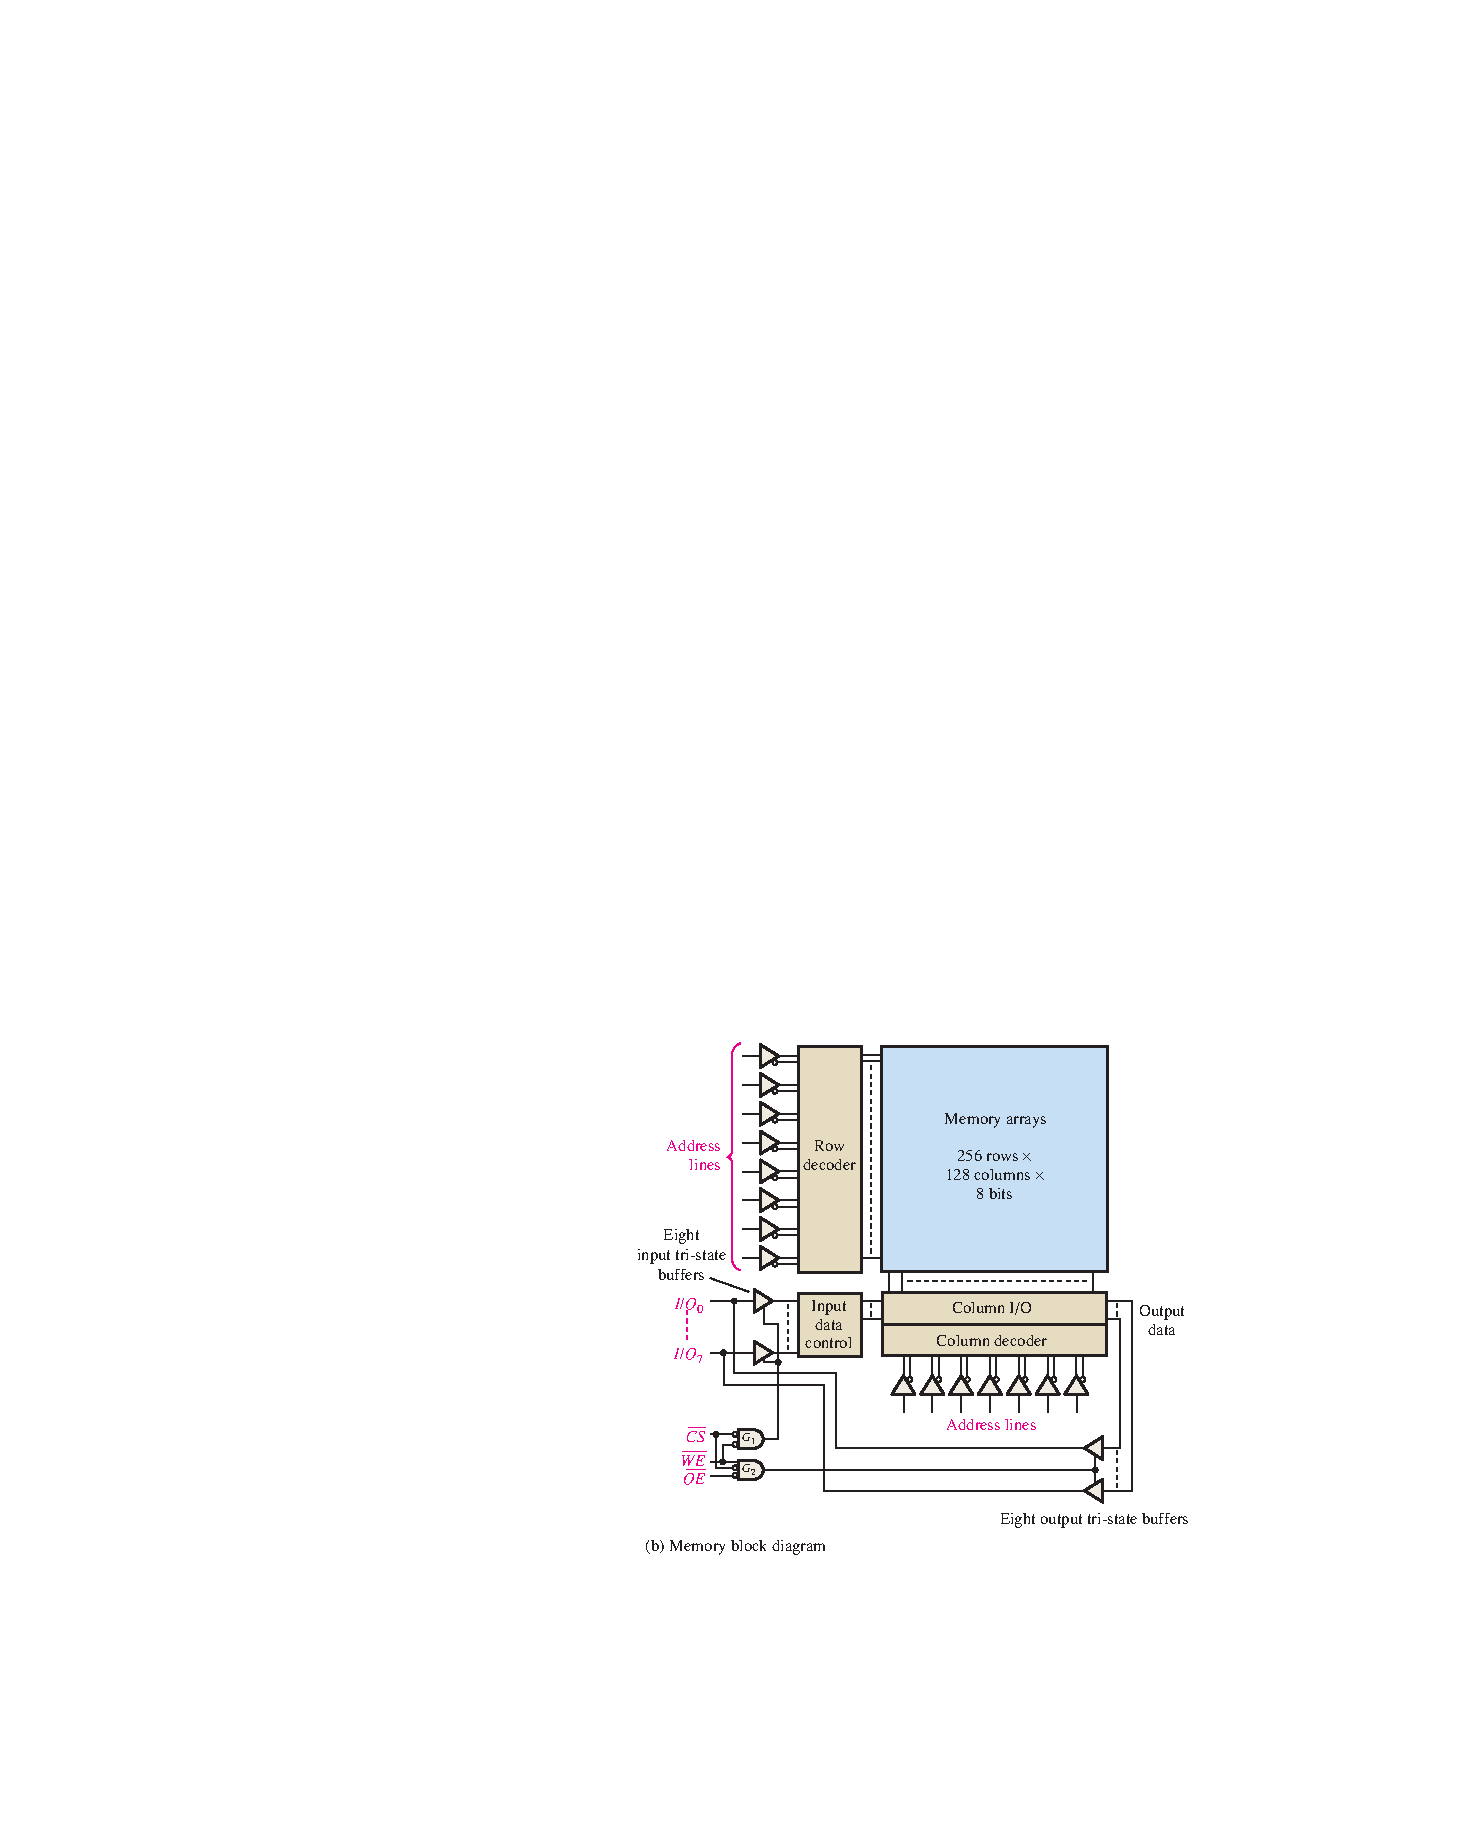
\includegraphics[scale = 0.85]{Graphics/RAM/RAM_BLOCK_DIAG.pdf}
    \caption{RAM block diagram ~\autocite{FLOYD}}
    \label{fig:RAM_BLOCK_DIAG}
\end{figure}


\begin{figure}[H]
    \centering
    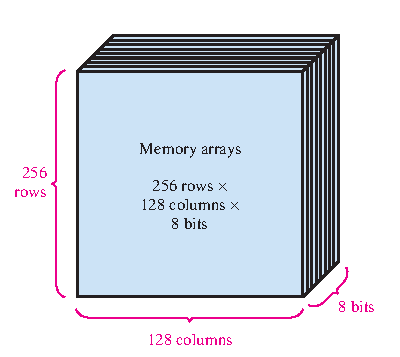
\includegraphics[scale = 0.85]{Graphics/RAM/RAM_BLOCK_CONFIG.pdf}
    \caption{RAM array configuration ~\autocite{FLOYD}}
    \label{fig:RAM_BLOCK_CONFIG}
\end{figure}


\subsubsection{Chip description}

\medskip
\hspace{0.5cm}
{\large \textit{\textbf{Chip Enable}}}
\medskip

To operate the memory first we have to activate the Chip Enable $\overline{CE}$  terminal (Active Low). \medskip

When a CPU has to handle multiple memory chips, in order to read or write from one of them, the other ones are disabled sending a HIGH to their respective $\overline{CE}$ terminals. 

\medskip
{\large \textit{\textbf{Write Enable}}}
\medskip

With this terminal the CPU specifies if the operation it wants to execute is to write into the memory (LOW at $\overline{WE}$) or to read from the memory (HIGH at $\overline{WE}$).

\medskip
{\large \textit{\textbf{Output enable}}}
\medskip


The $\overline{OE}$ connects the output of the memory to the data bus. If it is in LOW, data can be sent from the memory. Otherwise, a HIGH level will create a High-Z output at the Data Bus.  We usually keep it in a constant LOW in order to simplify the system.

\medskip
{\large \textit{\textbf{Address bus}}}
\medskip


In order to read or write, the GAL must first specify which memory location it wants to work with. This is done by means of the address bus, corresponding to the row and the column of the memory matrix. 

\begin{table}[H]
    \centering
        \begin{tabular}[t]{lccccc}
            \toprule
            & \textbf{Mode} & $\mathbf{\overline{CS}}$ & $\mathbf{\overline{OE}}$ & $\mathbf{\overline{WE}}$ & \textbf{I/O}\\
            \midrule
                &    Standby   &    H   &   X   &   X   &   High-Z        \\
                &    Read      &    L   &   L   &   H   &   $\text{DATA}_{OUT}$    \\
                &    Read      &    L   &   H   &   H   &   High-Z        \\
                &    Write     &    L   &   X   &   L   &   $\text{DATA}_{IN}$     \\
            \bottomrule
        \end{tabular}
        \caption{Operation Modes Truth Table ~\autocite{6116}}
        \label{table: RAM_MODES}
\end{table}


The RAM device used in the project is the 6116, a 16K (2048 x 8 bit) high speed memory chip.

In order to simplify the operation, as only 4 digits are stored, we will only use the A0 and A1 Address terminals. 

Also, as we only need to store digits from 0 to 9, only the first 4 bits of the Data Bus will be used.
